\documentclass{beamer}
\usepackage[T1]{fontenc}
\usepackage[utf8]{inputenc}
\usepackage{lmodern}

\usepackage{graphicx}
\graphicspath{{fig/}}

\newcommand*{\argmin}{\operatornamewithlimits{argmin}\limits}
\newcommand*{\argmax}{\operatornamewithlimits{argmax}\limits}

\usetheme{Copenhagen}

\title{Sound Source Localization and Seperation}
\author{Weipeng He \\ \texttt{2he@informatik.uni-hamburg.de}}
\date{June 6, 2013}

\begin{document}

\frame{\titlepage}

\begin{frame}
\frametitle{Outline}
\tableofcontents
\end{frame}

\section{Introduction}

\begin{frame}
\frametitle{Motivation}

\begin{itemize}
  \item Auditory perception is essential for animals.
  \begin{itemize}
    \item Localizing and tracking sound sources
    \item Predator and prey.
  \end{itemize}
  \item ``Cocktail Party Effect''
  \begin{itemize}
    \item Separation of sounds in a noisy environment.
  \end{itemize}
  ~
  \item Question : can machines do the same?
\end{itemize}
\end{frame}

\begin{frame}
\frametitle{Computational auditory scene analysis}
\begin{block}{Auditory scene analysis (ASA)}
    is a psychophysical study about the process by which the human auditory system organizes sound into perceptually meaningful elements.
  \end{block}
  ~
  \begin{block}{Computational auditory scene analysis (CASA)}
    is the study of auditory scene analysis by computational means. \\
    (``Machine listening'').
  \end{block}
\end{frame}

\begin{frame}
\frametitle{Computational auditory scene analysis}
\begin{block}{Input}
  (Multichannel) audio signal.
\end{block}
\begin{block}{Outputs}
  The direction of arrival and separated signal of each sound source.
\end{block}
\begin{itemize}
  \item CASA topics:
  \begin{itemize}
    \item Sound localization;
    \item Sound separation;
    \item Feature-based speech segregation;
    \item Analysis of musical audio signals;
    \item Noise (Reverberation) reduction;
    \item Acoustic simulation.
  \end{itemize}
\end{itemize}
\end{frame}

\begin{frame}
\frametitle{Applications}
\begin{itemize}
  \item Robotics
  \begin{itemize}
    \item Tracking of persons or interesting object
  \end{itemize}
  \item Hearing-aids, enhanced hearing
  \begin{itemize}
    \item Listening to selected sounds/conversations and improved speech intelligibility for hearing-impaired.
  \end{itemize}
  \item Mobile phones
  \begin{itemize}
    \item Environmental noise and interference suppression
  \end{itemize}
  \item Human-computer interfaces – speech recognition
  \begin{itemize}
    \item Pre-processing to improve signal-to-noise ratio
  \end{itemize}
  \item In-car and hands-free communication
  \begin{itemize}
    \item Noise and acoustic echo cancellation.
  \end{itemize}
\end{itemize}
\end{frame}

\begin{frame}
\frametitle{Comparison to visual system}
\begin{itemize}
  \item In robotics, auditory input is a complement of vision:
  \begin{itemize}
    \item additional modal;
    \item omnidirectional;
    \item does not require direct line-of-sight.
  \end{itemize}
  ~
  \item Difficulties:
  \begin{itemize}
    \item Time-variant;
    \item Noisy environment.
  \end{itemize}
\end{itemize}
\end{frame}

\section{Sound localization}
\begin{frame}
\frametitle{Sound localization in human}
\begin{itemize}
  \item Interaural time difference (ITD)
\end{itemize}
\begin{center}
  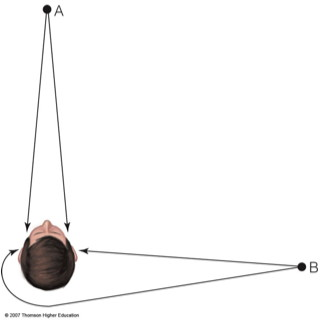
\includegraphics[width=.5\textwidth]{itd}
\end{center}
\end{frame}

\begin{frame}
\frametitle{Sound localization in human}
\begin{itemize}
  \item Interaural level difference (ILD)
\end{itemize}
\begin{center}
  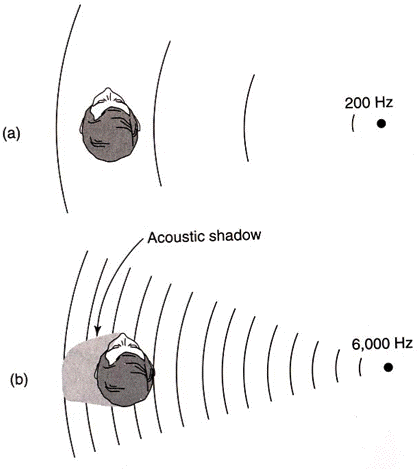
\includegraphics[width=.5\textwidth]{ild}
\end{center}
\end{frame}

\begin{frame}
\frametitle{Sound localization in human}
\begin{itemize}
  \item Outer Ear Vertical Localization
\end{itemize}
\begin{center}
  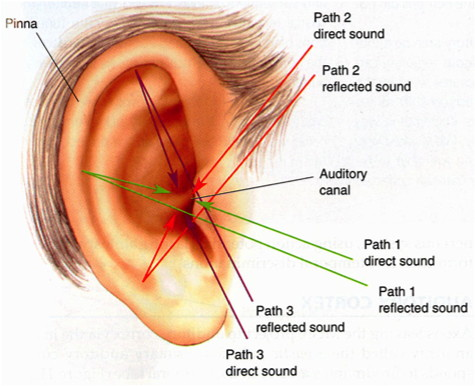
\includegraphics[width=.7\textwidth]{vertical}
\end{center}
\end{frame}

\begin{frame}
  \frametitle{Sound localization using ITD and cross-correlation\cite{murray_robotics_2004}}
  \begin{columns}
    \column{.6\textwidth}
\begin{center}
  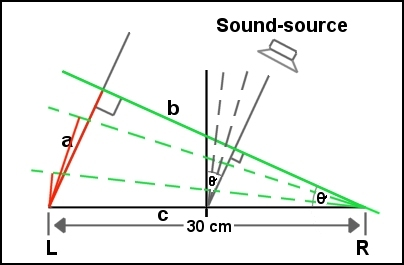
\includegraphics[width=\textwidth]{correl-007}
\end{center}
\column{.4\textwidth}
\[ sin(\theta) = \frac{\Delta d}{\overline{LR}} \]
\[ \Delta d = \Delta t \times v \]
\[ \theta = arcsin(\frac{\Delta t \times v}{\overline{LR}}) \]
  \end{columns}
\end{frame}

\begin{frame}
\frametitle{Sound localization using ITD and cross-correlation\cite{murray_robotics_2004}}
\begin{itemize}
  \item Using cross-correlation to calculate $\Delta t$:
  \[ Corr_j(g, h) = \sum_t g_{t+j} h{j} \]
  \[ \Delta t = R \times \argmax_{j} Coor_j(g, h) \]
  where $R$ is the sampling rate.
\end{itemize}
\end{frame}

\begin{frame}
\frametitle{Sound localization using ITD and cross-correlation\cite{murray_robotics_2004}}
\begin{center}
  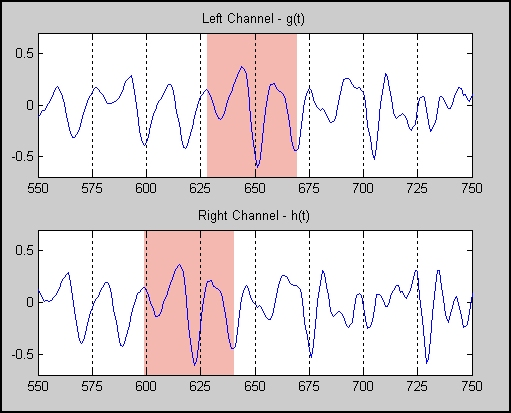
\includegraphics[width=.7\textwidth]{correl-003}
\end{center}
\end{frame}

\begin{frame}
\frametitle{Sound localization using ITD and cross-correlation\cite{murray_robotics_2004}}
\begin{center}
  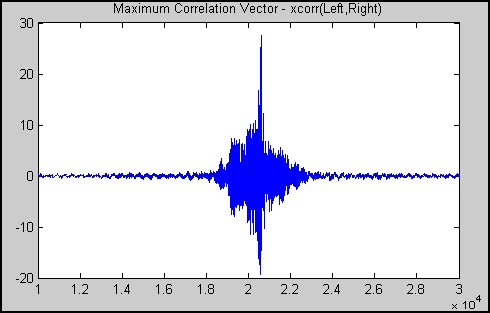
\includegraphics[width=.7\textwidth]{correl-006}
\end{center}
\end{frame}

\begin{frame}
\frametitle{Sound localization using ITD and cross-correlation\cite{murray_robotics_2004}}
\begin{columns}
    \column{.6\textwidth}
\begin{itemize}
  \item Results:
  \begin{itemize}
    \item Accuracy of $\pm 1.5^\circ$
    \item Human counterpart is $0.9 - 1.5^\circ$
  \end{itemize}
  \item Problems: 
  \begin{itemize}
    \item Time delay for calculation $1-2s$;
    \item Can't recognize front and back;
    \item Can only track a single source.
  \end{itemize}
\end{itemize}
    \column{.4\textwidth}
\begin{center}
  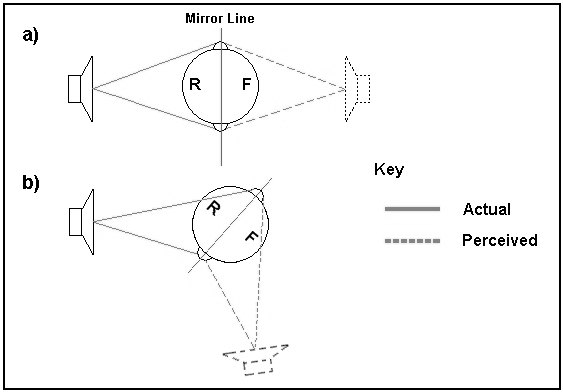
\includegraphics[width=\textwidth]{correl-008}
\end{center}
  
\end{columns}
\end{frame}

\begin{frame}
\frametitle{Improvement}
\begin{itemize}
  \item Mounting a bio-mimetic ear to the microphone and measure the itensity change;
  \item Using more microphones;
    \begin{itemize}
      \item Triangle;
      \item Circular;
      \item Linear;
      \item Irregular.
    \end{itemize}
  \item Using more complex algorithms:
    \begin{itemize}
      \item Time-frequency analysis;
      \item Intensity vector analysis.
    \end{itemize}
\end{itemize}
\end{frame}


\section{Sound separation}

\begin{frame}
\frametitle{Sound separation}
\begin{itemize}
  \item Sound separation is a problem closely related to source separation in digital signal processing.
  \item The auditory signal can be separated according to its feature.
  \item Its performance is improved by sound localization.
\end{itemize}
\end{frame}

\begin{frame}
\frametitle{Sound separation based on intensity vector statistics\cite{gunel_acoustic_2008}}
\begin{center}
  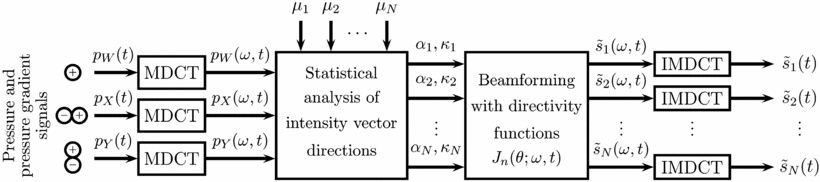
\includegraphics[width=\textwidth]{flow}
\end{center}
\end{frame}

\begin{frame}
\frametitle{Sound separation based on intensity vector statistics\cite{gunel_acoustic_2008}}
\begin{center}
  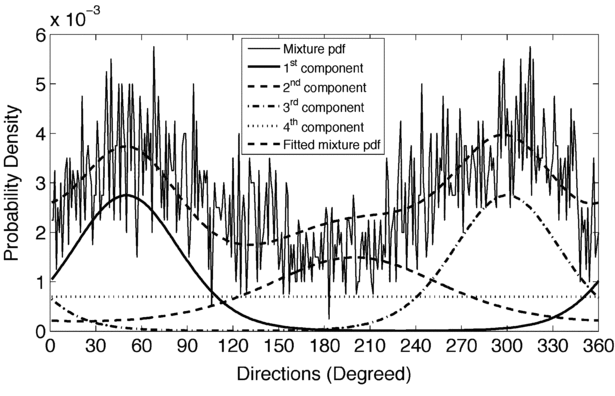
\includegraphics[width=.9\textwidth]{sep1}
\end{center}
\end{frame}

\begin{frame}
\frametitle{Sound separation based on intensity vector statistics\cite{gunel_acoustic_2008}}
\begin{itemize}
  \item Demo video.
\end{itemize}
\end{frame}

\section{Conclusion}

\begin{frame}
\frametitle{Conclusion}
\begin{itemize}
  \item Promising results have been shown in the study of sound localization and separation.
  \item These results can be applied to robotics and human-computer interaction.
\end{itemize}
\end{frame}

\section*{References}
\begin{frame}[allowframebreaks]
  \frametitle{References}
  {\footnotesize
  \bibliography{ref}
  \bibliographystyle{plain}  
  }
\end{frame}

\end{document}
